%!TEX root = ../main.tex


\centerline{\textbf{\xiaoer{本科毕业论文文献综述}}}
\bigskip

\textbf{摘要}\quad 
随着互联网的飞速发展,用户在线上所接触到的信息在复杂性和多样性等方面呈现出爆炸性增长的趋势。而推荐系统作为解决信息过载问题的一个切实有效的办法,在人们的日常生活中扮演着越来越重要的角色。同时,近些年来,深度学习在语音、图像还有自然语言处理等方面所取得的革命性的进展也越来越受到人们的关注。而相关的研究也表明:深度学习在信息检索和推荐等方面同样也有不错的表现。特别是亚马逊、YouTube等将深度学习应用到了自己网站的推荐系统上\cite{CovingtonAS16YouTube},并且取得了很好的效果。而这些也使得利用深度学习改进现有推荐算法成为当下研究的一个热点。
本文旨在在传统推荐方法的基础上,讨论推荐系统所面临的常见问题,以及深度学习在这些问题上的一些富有成果的研究,并对涉及到的相关深度学习技术进行具体的解释。


\chapter{背景}
在信息爆炸性增长的今天,个性化推荐系统已经成为人们生活中必不可少的筛选利器,并以多种多样的形式影响着人们生活的方方面面:亚马逊、淘宝等电商网站利用推荐引擎实时提供用户可能感兴趣的商品推荐;Twitter、Facebook等社交网站利用推荐系统为用户寻找潜在的好友推荐;Yotube、优酷等视频网站在用户观看视频的同时,利用推荐系统为用户提供最可能点击的视频推荐;Quora、今日头条等新闻门户网站则利用推荐系统帮用户筛选出最有价值的新闻。互联网广告利用推荐系统准确的找到潜在客户群,相比于随机投放提高了效率。推荐系统在促进商业发展以及便利人们决策等方方面面发挥着越来越重要的作用。

通常来说,推荐的内容列表一般是根据用户偏好、物品特征、用户与物品交互的历史记录以及一些诸如时间和空间数据这样的辅助信息而生成的。推荐系统的模型主要可以分为基于协同过滤的推荐、基于内容的推荐以及基于不同输入数据的混合推荐\cite{AdomaviciusT05}。然而这些模型在解决数据稀疏性(用户已评分的物品占总物品数量的很少一部分),冷启动问题(新的用户和新的物品往往没有评分数据)以及如何权衡不同指标下的推荐效果等问题上都有其各自的局限性。\cite{AdomaviciusT05}\cite{VekariyaK12Hybrid}\cite{McNeeRK06Being}\cite{VargasC11Rank}

在过去的十年间,我们已经见证了深度学习(Deep Learning)在诸如计算机视觉以及语音识别等领域的应用上,取得了显著的成功。而深度学习在解决很多复杂任务的良好效果,也促使学术界和工业界争相将其应用到其他更广阔的领域。最近,深度学习已经被逐渐应用到了推荐系统上\cite{CovingtonAS16YouTube}\cite{ChengKHSCAACCIA16Wide&Deep},改变了传统推荐系统的架构,并且在提升用户体验和满意度方面取得了令人瞩目的效果。一方面,通过学习一种深层次的非线性网络结构,深度学习可用来表征用户和物品相关的海量数据,利用这种强大的从样本中学习数据集本质特征的能力,可以获得用户和物品的深层次的特征表示。而另一方面,深度学习还能从诸如上下文、文本、图像等繁杂的数据中提取出数据之间错综复杂的内在关系,从而将不同数据映射到一个相同的隐空间,能够获得数据的统一表征\cite{PengZZXHLZHG17Cross-Media},在此基础上结合传统推荐方法来做推荐,可以有效利用多源异构数据,缓解传统推荐系统中的数据稀疏和冷启动问题。

推荐系统是工业领域中必不可少的一部分,在许多在线网站和手机应用中都为提升销量和服务发挥着不可忽视的作用。举例来说,人们在Netflix()中所观看的影片有$80\%$是来自于推荐\cite{Gomez-UribeH16Netflix},在YouTube上的视频点击有60\%是来源于推荐\cite{DavidsonLLNVGGHLLS10Youtube}最近,像Netflix、YouTube这样的公司也借助深度学习来提高推荐的质量\cite{ChengKHSCAACCIA16Wide&Deep}\cite{CovingtonAS16YouTube}\cite{OkuraTOT17Embedding}。比如Covington等人就提出了一种应用在YouTube上的借助于深度神经网络的视频推荐算法\cite{CovingtonAS16YouTube}。Cheng提出了一种应用在Google play App上的深广学习(wide\&deep)模型\cite{ChengKHSCAACCIA16Wide&Deep}。Shumpei则提出了一种应用在Yahoo新闻上的基于RNN的新闻推荐系统\cite{OkuraTOT17Embedding}。这些模型都已经在线上进行了测试,并且可以大幅度提高传统模型的推荐性能。可以预见的是,深度学习将引领推荐系统领域的一次巨大变革。

另一项令人瞩目的改变则发生在学术研究领域。近些年,基于深度学习的推荐算法的论文数量呈现出几何倍数的增长。
作为推荐系统领域的顶级会议,ACM推荐系统年会(ACM RecSys),在2016年就专门召开了第一届基于深度学习的推荐系统研究专题研讨会(DLRS'16),旨在促进基于深度学习的推荐系统在学术研究和工业应用的发展。由此可见,基于深度学习的推荐系统研究已经成为研究推荐系统的热点方向之一。

总而言之,不管是在学术研究还是工业应用,深度学习在推荐领域都已经取得了令人振奋成果。而要想在这一领域继续有所突破,理解和归纳前人研究模型的优缺点,必然是不可缺少的一项工作,而这也正是本文写作的目的所在。



% chapter 背景(end)

\chapter{传统推荐系统}
自从20世纪90年代,协同过滤技术被首次提出,推荐系统已经成为了一门独立的学科而受到了广泛的关注。作为推荐系统的核心,推荐算法主要是利用用户与物品之间的二元关系,基于用户历史行为记录或相似性关系来帮助发现用户可能感兴趣的项目。文献\cite{AdomaviciusT05}给出了推荐算法的形式化定义:用$U$表示所有用户(user)的集合,用$I$来表示所有物品(item)的集合。在真实系统中,$U$和$I$的规模通常非常大。这里我们定义一个效用函数$s$,用来计算物品$i$对用户$u$的推荐度,即$s:U \times I \rightarrow R$,其中$R$是一个全序的集合,而推荐算法所研究的主要问题就是通过推荐度的计算,为每一个用户$u \in U$找到最感兴趣的物品$i^{'} \in I$,如下所示:
\begin{equation}
\forall u \in U, i_u^{'} = arg \max_{i \in I} s(u,i)
\end{equation}		
在推荐系统领域,我们所需要解决的一个关键问题是如何将效用函数$s$从$U \times I$的一个子空间外推到整个$U \times I$空间。一般来说,我们用用户对物品的评分来表示推荐度,而在真实的推荐系统中,用户往往只评分了其中的一小部分项目。因此,在推荐给用户最感兴趣的物品之前,必须先根据已知评分对未知评分进行预测,这就是我们之前所说的外推过程。根据对未知评分预测方法的不同,传统的推荐算法通常可以分成以下三种\cite{VerbertMOWDBD12ContextAware}:基于内容的推荐(content-based recommendation)、协同过滤推荐(collaborative filtering recommendation)和混合推荐(hybrid recommendation)。
\section{主要算法介绍}
\subsection{基于内容的推荐}
基于内容的过滤方法为每个用户或物品创建描述以表征其性质,例如,电影的描述可以包括其类型、导演、票房等方面,用户的描述可以是个人资料或从已评分物品中识别出的共同特征。这样就能计算出用户与待测物品在内容上的匹配度,进而根据匹配度对所有需要预测的物品进行排序,最终为用户推荐其潜在感兴趣的物品。
% subsection 基于内容的推荐(end)
\subsection{协同过滤推荐}
协同过滤利用相似用户之间具有相似兴趣偏好的规律,来发现用户对物品的潜在偏好。举个例子来说,基于用户的协同过滤算法(User-based Collaborative Filtering)会搜索那些与目标用户具有相似评分模式的用户作为相似用户,然后利用这些兴趣相投的相似用户的评分来预测其他未评分物品的评分。而基于物品的协同过滤算法(Item-based Collaborative Filtering)则是从物品的角度出发来预测评分。它首先计算一个物品-物品的相似矩阵,来确定每一对物品之间的相似度。然后再根据目标用户对相似物品已有的评分,来预测目标用户对未评分产品可能的评分。
% subsection 协同过滤推荐(end)
\subsection{混合推荐}
混合推荐通过组合不同推荐算法,往往能相比单一推荐算法,产生更好的性能。举例来说,可以以协同过滤算法为框架,结合基于内容的推荐算法来环节数据稀疏问题,这属于模型层面上的混合推荐。也可以将所有用户属性、用户行为等数据作为输入,通过训练一个统一的分类器来产生推荐结果,这属于特征层面上的混合推荐。
% subsection 混合推荐(end)
% section 主要算法介绍(end)
\section{传统算法存在的问题}
协同过滤算法是目前应用最为广泛的推荐算法,但往往面临数据稀疏和冷启动等问题。此外,经典的协同过滤算法采用的浅层模型往往无法学习到用户和物品更深层次的特征。基于内容的推荐算法可有效缓解数据稀疏和新物品的冷启动问题,但相应的,这种算法依赖于有效的特征提取,而传统的浅层模型往往需要人工设计特征,其有效性和可扩展性非常有限。近些年来,蕴含用户丰富个性化需求信息的文本、图像、标签在内等多源异构数据被越来越多地加入到了传统的推荐算法中。而融合了多源异构辅助信息(side information)的混合推荐算法也越来越被人们所重视,在解决数据稀疏和冷启动问题上具有不错的效果。但是由于辅助信息往往具有多模态、数据异构、大规模、数据稀疏和分布不均匀等复杂特征,融合多源异构数据的混合推荐方法研究依然面临着严峻的挑战\cite{WangWY15CDL}\cite{ZhangYLXM16CKBE}。
% section 传统算法存在的问题(end)
% chapter 传统推荐系统(end)

\chapter{基于深度学习的推荐系统}
\section{深度学习技术}
深度学习属于机器学习的一个子领域,它从数据中学习到不同层次的数据表示和抽象,可以用来解决有监督和无监督学习任务\cite{DengY14DLMA}。本节中,我们主要介绍一些和推荐系统领域密切相关的深度学习技术。

\subsection{多层感知机(Multilayer Perceptron, MLP)}
多层感知机(MLP)是一种前馈神经网络,与传统的只有输入层和输出层的感知机不同,它在输入和输出层之间加入一个或多个隐藏层。因此,多层感知机可以灵活应用激活函数(activation function)使其不仅仅局限于二分类问题。

这里以一个最简单的只含有一个隐藏层的MLP为例\cite{abs-1801-07883DLS}:
\begin{figure}[h]
\centering
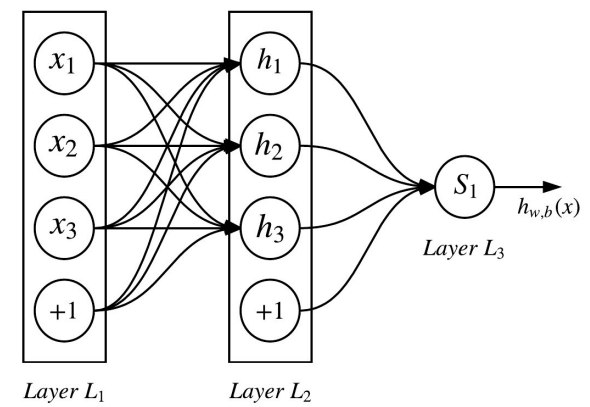
\includegraphics[width=0.5\linewidth]{images/MLP.png}
\caption{只含有一个隐藏层的MLP}
\label{fig:fig1}
\end{figure}
我们用一个$3$维向量$X=[x_1,x_2,x_3]$表示图中输入层,用$3$维向量$H[h_1,h_2,h_3]$表示图中隐藏层.则有$H = f(W^{T}X) = f(\sum\nolimits_{i=1}^{3}W^{1}_{i}x_{i} + b^{1})$其中$W^{1}$是第一层的$3 \times 3$的权重矩阵,$f$是激励函数,$b^{1}$是第一层的偏置项(bias)。这里激励函数$f$通常是非线性的,一般选用$sigmoid$函数、$tanh$函数或者$ReLU$函数。代入之后,表达式分别如下所示:
\begin{equation}
f(W^TX) = sigmoid(W^TX) = \frac{1}{1+exp(-W^TX)}
\end{equation}

\begin{equation}
f(W^TX) = tanh(W^TX) = \frac{e^{W^TX} - e^{-W^TX}}{e^{W^TX} + e^{-W^TX}}
\end{equation}

\begin{equation}
f(W^TX) = ReLU(W^TX) = \max(0,W^TX)
\end{equation}
而由隐藏层到输出层则可以看成是一个多类别的逻辑回归,一般选用$softmax$函数作为激励函数。则输出可以表示为$softmax(\sum\nolimits_{i=1}^{3}W^{2}_{i}x_{i} + b^{2})$,这里$W^{2}$是第二层的$3 \times 3$的权重矩阵,$f$是激励函数,$b^{2}$是第二层的偏置项(bias)。
总结起来,这个三层MLP用公式总结起来就是
\begin{equation}
g(X) = G(b^{2} + W^{2}(f(b^{1} + W^{1}X)))
\end{equation}
其中函数$G$就是softmax函数,它将多个神经元的输出映射到(0,1)区间内,一般用来进行多分类。$softmmax$函数定义如下:
\begin{equation}
G(X)_j = \frac{e^{x_j}}{\sum\nolimits_{k=1}^{K}e^{x_k}}	\qquad  for \quad j = 1,...,k
\end{equation}
这里$K$代表输入变量$X$的维度。
\subsection{自动编码器(Autoencoder,AE)}
自动编码器依靠编码和解码过程来重构输入数据,从而学习数据的隐层表示。传统的自动编码器可以视为一个三层的神经网络:包含有相同规模的输入层$x$和输出层$y$,还有一个隐藏层$h$,其结构如下图所示。

\begin{figure}[htbp]
\centering
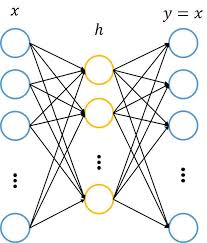
\includegraphics[width=0.22\linewidth]{images/AE.jpg}
\caption{自动编码器结构示意图}
\label{fig:fig2}
\end{figure}

自动编码器的目的是使得输入$x$和输出$y$尽可能接近,并用重构误差来表示这种接近程度。一般重构误差包括均方误差(mean-square error, MSE)和交叉熵(cross-entropy)。
为了解决自动编码器容易学习到一个恒等函数的问题,研究者后来又提出了稀疏自动编码器和降噪自动编码器。2007年,Bengio等人\cite{VincentLBM08Bengio}通过堆叠多个降噪自动编码器,提出了栈式降噪自动编码器(Stacked Denoising Autoencoder, SDAE)的概念。
如今,自动编码器,特别是栈式降噪自动编码器,在推荐系统中主要被用于学习用户和项目的隐层表示,通过重构学习用户和物品的相关信息(如评分数据和文本、图像信息),从而获得用户或物品的隐层表示,最后基于这种隐层表示来预测用户对物品的偏好,并应用在评分预测、文本推荐和图像推荐等场景中\cite{WangSY15SDAE}。
\subsection{卷积神经网络(Convolutional Neural Network,CNN)}
卷积神经网络是当今图像识别领域的研究热点。相比于传统的MLP,卷积神经网络使用池化(pooling)可以减少模型中的神经元数量。特别是当输入层是多维图像的时候,CNN可以将图像直接作为网络的输入,从而可以避免传统处理算法中复杂的特征提取和数据重建过程。卷积神经网络的基本结构主要分为输入层、卷积层、下采样层(池化层)、全连接层和输出层,如下图所示。

\begin{figure}[htbp]
\centering
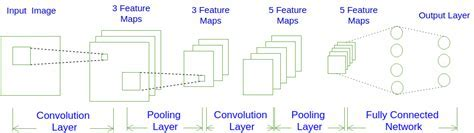
\includegraphics[width=0.5\linewidth]{images/CNN.jpg}
\caption{卷积神经网络结构示意图}
\label{fig:fig3}
\end{figure}

在推荐系统领域,CNN主要被用来从文本、图像、音频等内容中提取物品的隐藏特征,从而获取物品的低维向量表示,其在音乐推荐、图像推荐还有文本推荐等领域都有所应用\cite{GengZBC15IMAGE}。
\subsection{循环神经网络(Recurrent Neural Network,RNN)}
传统CNN的层与层之间是全连接的,而每一层的节点之间则没有连接。与之不同的是,循环神经网络在网络各隐层的节点之间加入连接,从而能够通过获取输入层的输出和前一时刻的隐层状态来计算当前时刻隐层的输出,也就是说RNN能够对过去的信息进行记忆。下图是一个包含输入单元、输出单元和隐层单元的典型RNN结构。

\begin{figure}[htbp]
\centering
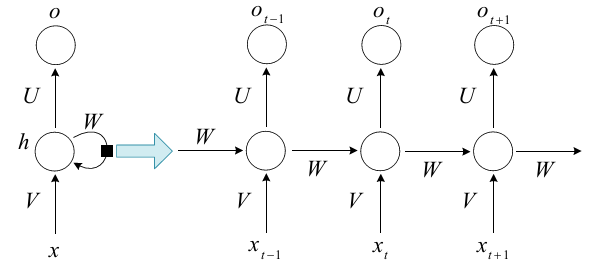
\includegraphics[width=0.5\linewidth]{images/RNN.png}
\caption{循环神经网络结构示意图}
\label{fig:fig4}
\end{figure}

而为了解决传统RNN存在梯度消失和难以学习数据之间的长期以来关系的问题,Hochreiter等人\cite{HochreiterS97LSTM}提出了长短时间记忆网络(Long Shor-Term Memory, LSTM),Cho等人\cite{ChoMBB14GRU}则提出了门限循环单元(Gated Recurrent Unit,GRU)。LSTM和GRU通过增加保存长期状态的隐层单元,能够更加有效地建模长期以来关系,是目前应用最为广泛的循环神经网络模型。
在推荐系统领域,RNN主要用来建模数据之间的序列影响,从而帮助获取更为有效的用户和物品隐层表示。一方面,RNN可以被用来建模推荐系统中用户行为的序列模式\cite{WuABSJ17RRN}\cite{SongEH16DL4TR},另一方面,它还可以被应用在建模用户和物品相关的文本信息中词语之间的序列影响\cite{0014SY16CRA}\cite{0014SY16CRA}。在文本推荐、图像推荐、评分预测以及基于未知社交网络中的兴趣点推荐等领域应用广泛。
\subsection{受限制玻尔兹曼机(Restricted Boltzmann Machine,RBM)} 
玻尔兹曼机(Boltzmann machine, BM)由一些二元的可见单元(对应可见变量,即数据样本)和一些二元的隐层单元(对应隐层变量)构成。当处于状态0,表示该神经元处于抑制状态,而状态1则对应表示该神经元处于激活状态。虽然BM具有强大的无监督学习能力,但其训练过程却非常耗时。为此,Sejnowski等人提出了受限制玻尔兹曼机(Restricted Boltzmann Machine, RBM),通过在原有BM基础上除去同层变量之间的连接,可以显著提高学习效率。
如下图所示,RBM包括可见层$v$以及隐层$h$,两层之间是全连接的,而同层的节点之间则是互不连接的。

\begin{figure}[htbp]
\centering
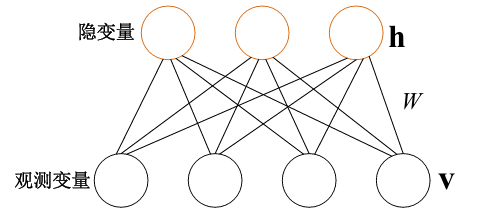
\includegraphics[width=0.5\linewidth]{images/RBM.png}
\caption{受限制玻尔兹曼结构示意图}
\label{fig:fig5}
\end{figure}

作为最早被应用在推荐系统中的神经网络模型\cite{MelloZS07aRBMCF}\cite{TruyenPV09BMCF},RBM当前主要用来重构用户的评分数据,从而学习到用户的隐层表示,进而实现对未知评分的预测。
% section 深度学习技术(end)

\section{深度学习在推荐领域的研究现状}
深度学习当前在推荐系统中,主要用来学习用户和物品的输入数据从而获得隐层表示,然后再根据这种隐层表示为用户推荐物品。一个基于深度学习的推荐系统框架,如下图所示通常包含三层:输入层、模型层还有输出层。

\begin{figure}[htbp]
\centering
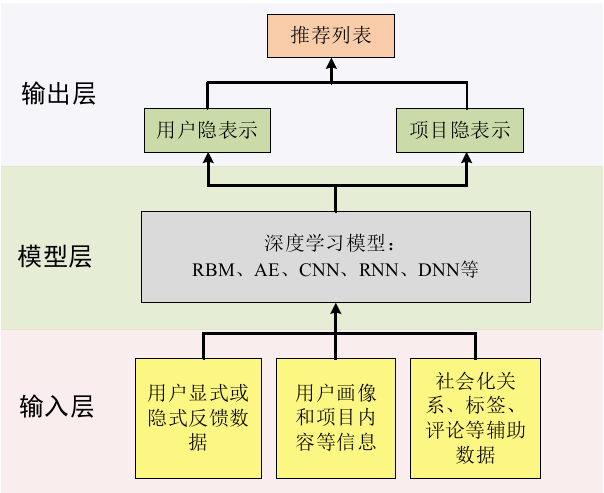
\includegraphics[width=0.5\linewidth]{images/DLframework.png}
\caption{基于深度学习的推荐系统框架}
\label{fig:fig1}
\end{figure}

输入层的数据一般包括:用户的显式反馈(评分、喜欢或不喜欢)或隐式反馈数据(浏览、点击等行为数据)、用户画像(性别、年龄、偏好等)和物品内容(文本、图像等信息)、用户生成内容(社会化关系、标签、评论等辅助数据)。在模型层,通常使用前面提到的深度学习技术(如受限制玻尔兹曼机、自动编码器、卷积神经网络、循环神经网络等)来处理输入数据并获得隐层表示。而在输出层,则将得到的隐层表示通过内积(inner product)、Softmax、相似度计算等方法产生项目的推荐列表。

\subsection{深度学习在基于内容的推荐系统中的应用}
在基于内容的推荐系统中,深度学习可以用来从项目的内容信息中提取物品的隐层表示,以及从用户的画像信息以及历史行为数据中获取用户的隐层表示,之后再基于获得的隐层表示来计算书用户和物品的匹配度,进而为用户推荐物品。

1)基于MLP的内容推荐

Cheng等人\cite{ChengKHSCAACCIA16Wide&Deep}通过学习用户特征、物品特征和情境特征等多源异构数据,提出了用于APP推荐的深广学习(Wide\&Deep Learning)模型。如下图所示,该模型联合训练了一个宽广线性模型(图中左侧)和一个深度神经网络(图中右侧)来确保模型记忆能力和泛化能力的均衡。

\begin{figure}[htbp]
\centering
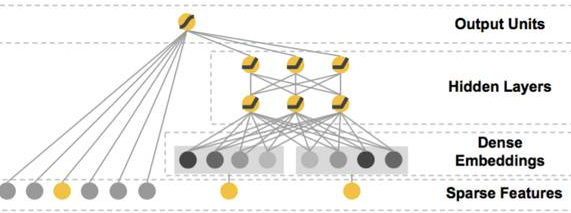
\includegraphics[width=0.5\linewidth]{images/WideDeep.png}
\caption{深广学习模型结构}
\label{fig:fig1}
\end{figure}

与深广模型类似,He等人\cite{abs-1708-05031NCF}提出了一种神经协同过滤方法(Neural Collaborative Filtering,NCF),该方法通过将用户和物品的的特征作为输入,并利用多层神经网络来学习用户和物品之间的交互函数,得到一种矩阵因子分解的泛化结构和一种多层感知机结构。接下来利用神经矩阵因子分解模型(Neural Matrix Factorization Model,NeuMF)来组合矩阵因子分解的线性特征和深度神经网络的非线性特征。除此之外,Covington等人\cite{CovingtonAS16YouTube}也提出了一种基于MLP的深度神经网络模型,并应用在了YouTube视频推荐上。

2)基于CNN的内容推荐

Gong等人\cite{GongZ16HashtagAttention}提出了一种基于注意力的卷积神经网络(Attention-based Neural Network)来进行微博中的Hashtag推荐。这里,作者将hashtag推荐问题理解为一个多标记分类问题,并用CNN来获取微博的特征。之后,Zhang等人\cite{ZhangWHHG17HashtagMulti}通过利用多模信息来进行微博的hashtag推荐。这里,作者采用CNN从图像中提取特征,而用RNN从文本中提取特征,之后再结合这两方面的特征来进行标签推荐。而注意力机制则用来建模图像和文本信息的局部关联性。除此之外,Wang等人\cite{WangYRTZYW17ArticleRec}则利用CNN来学习文章中的语义信息,提出了一种动态注意力深度模型(Dynamic Attention Deep Model,DADM),用来研究编辑者的文章推荐问题。Oord等人\cite{OordDS13MusicRec}则利用CNN来学习音乐的音频信号数据和用户的历史收听数据,来解决音乐推荐系统中的冷启动问题。

3)基于RNN的内容推荐

与基于注意力的CNN模型类似,注意力机制也被用于基于RNN的内容推荐中。Li等人\cite{LiLJZ16HashtagRNN}就提出了一种基于注意力的LSTM模型来进行微博中的hashtag推荐。将RNN与注意力机制结合起来,可以帮助提取文本中的序列特征,从而在微博中识别出最具有信息量的词。同时,RNN还经常被用来做新闻推荐,Okura等人\cite{OkuraTOT17NewsRecRNN}就首先使用降噪自动编码器(DAE)来从新闻中提取出文章的隐层表示,并采用RNN来从用户的历史行为列表中来学习用户的隐层表示,从而来获取用户偏好,之后将基于新闻和用户的隐层表示用点乘进行关联,最终为用户产生新闻推荐列表。

\subsection{深度学习在协同过滤中的应用}
将深度学习应用于协同过滤中,可有效改善传统矩阵因子分解可扩展性不足的问题\cite{SalakhutdinovMH07RBM}。其通常做法一般是,将用户的评分向量(或者是物品的被评分向量)作为输入,利用深度学习来学习用户或物品的隐层表示,之后再利用逐点损失(Point-wise Loss)和成对损失(Pair-wise Loss)等损失函数来对模型的参数进行优化\cite{WuDZE16CDAE},最后再用学习到的隐层表示来进行物品推荐。

1)基于AE的协同过滤

自动编码器近些年来,被越来越多地应用到了传统的协同过滤方法中。如Sedhain等人\cite{SedhainMSX15AECF}提出的基于自动编码器的协同过滤模型(AutoRec),就利用自动编码器的编码过程和解码过程来产生输出,并通过最小化重构误差来优化模型的参数,进而对评分进行预测。而与AutoRec不同的是,Strub等人\cite{CFSDAE}利用两个栈式降噪自动编码器(SDAE),针对评分矩阵的稀疏性问题,在训练过程中直接将评分矩阵中的缺失值归零,从而减少了网络的连接数量。Wu等人\cite{WuDZE16CDAE}的协同降噪自动编码器(Collaborative Denoising Auto-Encoders,CDAE)则是将自动编码器应用到了top-N推荐问题上。

2)基于RBM的协同过滤

Salakhutdinov等人\cite{TruyenPV09BMCF}在2007年最早将受限制玻尔兹曼机应用到协同过滤推荐模型之中。针对传统RBM模型仅仅利用物品之间的关联关系,Georgiev等人\cite{GeorgievN13NONIID}在原有RBM模型基础上进行了扩展,并且简化了模型的训练和预测过程。后来,何洁月等人\cite{HeJieYue}又将好友信任关系加入到RBM之中,提出一种基于实值状态的玻尔兹曼机,有效缓解了原有模型的稀疏性问题。

3)基于RNN的协同过滤

RNN能够建模用户行为之间的相互依赖关系,也可以用来建模用户的历史行为对当前时刻用户行为的影响。因此可以利用RNN,在传统协同过滤之中融入时间序列信息,从而提升推荐系统的性能。为此,Song等人\cite{SongEH16DL4TR}通过融入时间信息并在多种粒度上建模用户的兴趣偏好,提出了一种多等级时间深度语义结构化模型(Mutli-Rate TDSSM)。而考虑到推荐系统中的用户行为之间往往存在着多种类型,Liu等人\cite{LiuWW17RLBL}提出了一种循环Log双线性模型(Recurrent Log-BiLinear,RLBL),该模型用RNN来建模用户行为之间的长程依赖关系,而用Log双线性模型(Log-BiLinear,LBL)\cite{MnihH07LBL}来建模短时的情境信息,从而对用户在下一时刻的行为信息进行预测。

\section{基于深度学习的推荐系统的优势和存在的问题}
基于深度学习的推荐系统能够有效地融合多源异构数据,可以缓解传统推荐系统中的数据稀疏和冷启动问题。而融合多种推荐方法的混合推荐,虽然也可以在一定成都上缓解数据稀疏问题,但是这种方法却面临着辅助数据难以表示的问题。传统的方法,如协同主题回归(Collaborative Topic Regression,CTR)\cite{WangB11CTM},并不能获取辅助数据的有效表示\cite{WangWY15CDL}。而利用深度学习来自动提取特征,则可以从辅助数据中学习到有效的用户和物品隐层表示。
\subsection{优势}
总的来说,相比于传统推荐方法,基于深度学习的推荐方法一般有以下三点优势:

1)传统浅层模型提取到的特征通常是稀疏和高维的,而深度学习可以学习到非线性的多层次抽象特征表示,获取稠密和低维的特征表示\cite{ChengKHSCAACCIA16Wide&Deep}。

2)深度学习可以克服不同数据之间的异构性\cite{ZhangYLXM16CKBE}\cite{CovingtonAS16YouTube},可以方便地通过各种粗糙的原始数据的输入来学习到用户和物品的隐层表示。

3)深度学习可以帮助从图像、视频这样的非结构化中提取特征信息,避免复杂的人工特征工程\cite{ZhangYLXM16CKBE}。
\subsection{存在的问题}
同时,基于深度学习的推荐方法往往也存在着以下问题:

1)可解释性问题。基于深度学习的推荐模型往往类似于一个黑盒,难以为最终做出的推荐结果找到一个合理的解释。而如何在增强深度学习在推荐系统中的可解释性,仍需要进一步的深入研究。

2)可扩展性问题。深度学习在推荐系统中的另一个难题在于,其模型往往需要长时间的训练,而权衡模型的可扩展性与复杂度仍是当前的一大挑战。


% section 深度学习在推荐领域的研究现状(end)
% chapter 基于深度学习的推荐系统(end) 

\chapter{总结与展望}
本文在传统推荐方法的基础上,介绍了当前基于深度学习的推荐系统的研究现状,并对其中涉及到的深度学习技术做了具体的说明。通过上面的总结,可以看到,深度学习在推荐系统领域的应用目前仍然处于起步阶段,接下来必将会有更多、更广泛的尝试\cite{ZhangYS17aaSurveyPerspect}。
而对于未来的发展趋势,则可以从以下三个方面进行展望:

1)将深度学习与现有推荐方法相结合

基于内容的方法和协同过滤方法等传统方法的研究已经日臻完善。而且普遍具有实现方便和可解释性强等优势。而深度学习则可以融合用户评论、标签信息以及社交关系等多源异构数据,学习到用户和物品更深层次的表示。而结合两者的优势,将深度学习与传统推荐方法相结合的研究,也将会是未来研究的发展趋势。

2)基于深度学习的跨域推荐

融合用户在不同平台的数据,从而进行跨域推荐,可以克服单一领域信息不足,并有利于缓解数据稀疏和冷启动问题。目前针对跨域推荐,当前主要的研究方法包括基于协同过滤的方法、基于迁移学习的方法和基于张量分解的方法等。但这些方法通常只能针对特定的信息进行融合,适应性和可扩展性有待提升。而结合深度学习的跨域推荐则方便融合不同类型的异构数据进行推荐,且目前已经在Google\cite{CovingtonAS16YouTube}和微软\cite{WuABSJ17RRN}等公司得到了实际应用。基于深度学习的跨域推荐,也将是未来的研究重点。

3)可解释性方面的研究

基于深度学习的推荐方法在提供给用户推荐结果的同时,往往难以给出合理的推荐理由,这在一定程度上会减低用户对推荐结果的接受程度。因此在未来,有必要从模型、数据还有心理学、经济学等方面进行研究,来提升深度学习推荐结果的可解释性。\cite{王国霞2012个性化推荐系统综述}

% chapter 总结与展望(end)


\bibliography{data/survey}




